\documentclass{jarticle}
\pagestyle{empty}
\usepackage{graphicx}
\usepackage{booktabs}
\setlength{\topmargin}{-10.4mm}
\setlength{\headheight}{0mm}
\setlength{\headsep}{0mm}
\setlength{\textheight}{262mm}
\setlength{\textwidth}{180mm}
%\setlength{\topskip}{7mm}
\setlength{\evensidemargin}{-10.4mm} 
\setlength{\oddsidemargin}{-10.4mm} 
\setlength{\columnsep}{8mm}
% \setlength{\footskip}{12mm}
\usepackage{subfigure}
\usepackage{color}
\usepackage{setspace}
\usepackage{url}
\usepackage {signchart}

% 行間調整
\setstretch{0.9}

%sectionのフォントサイズ修正
\makeatletter
\def\section{\@startsection {section}{1}{\z@}{2.5ex plus -1ex minus -.2ex}{1.3 ex plus .1ex}{\large\bf}}
\makeatother 

%subsectionのフォントサイズ修正
\makeatletter
\def\subsection{\@startsection {subsection}{1}{\z@}{1.5ex plus -1ex minus -.4ex}{0.3 ex plus .1ex}{\bf}}
\makeatother 

\begin{document}
\twocolumn[

\begin{center}
%タイトル
{\LARGE \textbf{\\認知症予防トレーニングの負荷調整システムに関する研究}}\\
%サブタイトル
%{\Large \textbf{必要に応じてサブタイトル}}
\end{center}

\begin{center}
% 著者
\begin{tabular}{cccc}
% 1名の場合
\multicolumn{4}{c}{X13001 相羽瑛仁}\\
% 2名の場合
%& K11002 愛工七音 & X11003 愛工頼音 &\\
% 3名の場合
%K11001 愛工総和 & K11002 愛工今鹿 & X11003 愛工姫星&\\
% 4名の場合
%K11001 愛工総和 & K11002 愛工今鹿 & X11003 愛工姫星& X11004 愛工緑輝\\
% 指導教員
\multicolumn{4}{c}{\textbf{指導教員} 澤野弘明}
\end{tabular}
\hspace{2zw}
\end{center}
]

%--------------------------------------------
\section{はじめに}
高齢者向けの運動教室で実施されるトレーニングの一つにコグニサイズ(cognicise)がある\cite{コグニサイズとは}.コグニサイズは認知症予防を目的としたトレーニングであり,運動と同時に,計算やしりとりなどの認知課題を行う.コグニサイズは実施する運動と認知課題に応じて,コグニステップ,コグニラダー,コグニウォークなどの種類がある.文献\cite{コグニサイズとは}では,認知症予防の効果があるコグニサイズの条件として,1)運動は全身を使った中強度程度の負荷がかかるものであり,脈拍数が上昇する,2)運動と同時に実施する認知課題によって,運動の方法や認知課題自体をたまに間違えてしまう程度の負荷がかかっているとしている.また文献\cite{コグニサイズとは}では,個人の身体状況に応じて,運動と認知課題の負荷を調整することが重要だとしている.しかし,運動教室で実施される集団でのコグニサイズは,参加者全員に対する負荷が一定のため,認知症予防の効果が低い参加者が現れる可能性がある\cite{運動教室の効果}.

北越の研究\cite{認知課題ゲーム}では,タブレット端末上に自律的に動作するエージェントを実装し,高齢者がエージェントとの認知課題ゲームに取り組むことで,認知機能の向上を支援するシステムを開発している.認知課題の視覚的フィードバックを導入することで,高齢者が認知課題に取り組むモチベーションの向上に効果があると報告されている.

そこで本研究では,ICTを使用し,運動教室で実施される集団でのコグニサイズにおいて,認知課題の負荷を個別に調整する支援を行う.認知課題の正答率を蓄積し,蓄積した認知課題の正答率に応じて,認知課題の負荷を調整可能なシステムを開発する.運動教室の参加者が提案システムを使用することによって,個別に認知症予防の効果があるコグニサイズを実施できることが期待される.また,提案システムに認知課題の視覚的フィードバックを導入することで,参加者のモチベーションの向上が期待される.本稿では,運動教室の参加者に対して提案システムへ抱く印象についてのアンケート評価を行った.


% 運動教室でのコグニサイズの実施の様子を図\ref{fig:20171207_cognicise}に示す.
\if0
\begin{figure}[b]
\begin{center}
\includegraphics[width=.40\textwidth]{20171207_cognicise.eps}
\caption{運動教室でのコグニサイズの実施の様子}
\label{fig:20171207_cognicise}
\end{center}
\end{figure}
\fi

%--------------------------------------------
\section{提案システム}
本節では,運動教室で実施される集団でのコグニサイズにおいて,認知課題の負荷を個別に調整可能なシステムを提案する.本稿では,コグニサイズの一つであるコグニステップに対応した提案システムを開発する.コグニステップは,数字を数えながら左右の足で交互にステップをする運動と同時に,一定間隔ごとの決められた数字のときに拍手をする認知課題を行う.コグニステップの認知課題の負荷は,拍手をする数字の間隔を変更することで調整可能である.提案システムは,認知課題の負荷を個別に調整するために,認知課題の正答率を蓄積する.また,参加者のモチベーションの向上のために,認知課題の視覚的フィードバックを行う.提案システムの構成図を図\ref{fig:system}に示す.

認知課題の正答率を蓄積するために,身体動作の認識が可能なKinectを使用し,認知課題の拍手動作を検出する.検出した拍手動作を利用し,認知課題の正誤判定を行う.認知課題の正誤判定をコグニステップ実施中に集計し,コグニステップ終了後に集計結果から認知課題の正答率を算出する.算出した認知課題の正答率はPC上のデータベースに蓄積する.

認知課題の視覚的フィードバックを行うために,Kinectに内蔵されるRGBカメラで参加者を撮影し,撮影した動画を参加者の正面にプロジェクタで投影する.プロジェクタ投影面には図\ref{fig:projection_surface}で示すように,認知課題を個別に表示する.表示する認知課題はPC上の管理画面で個別に変更可能である.図\ref{fig:system_management}にPC上の管理画面を示す.データベースに蓄積した認知課題の正答率を図\ref{fig:check_answer_rate}で示すPC上の管理画面で確認し,認知課題の正答率に応じて認知課題を個別に変更する.参加者がプロジェクタ投影面に表示される認知課題のコグニステップを実施することで,認知課題の負荷を個別に調整する支援とする.

\begin{figure}[tbp]
\begin{center}
\includegraphics[width=.40\textwidth]{system.eps}
\caption{システム構成図}
\label{fig:system}
\end{center}
\end{figure}

\begin{figure}[tbp]
\begin{center}
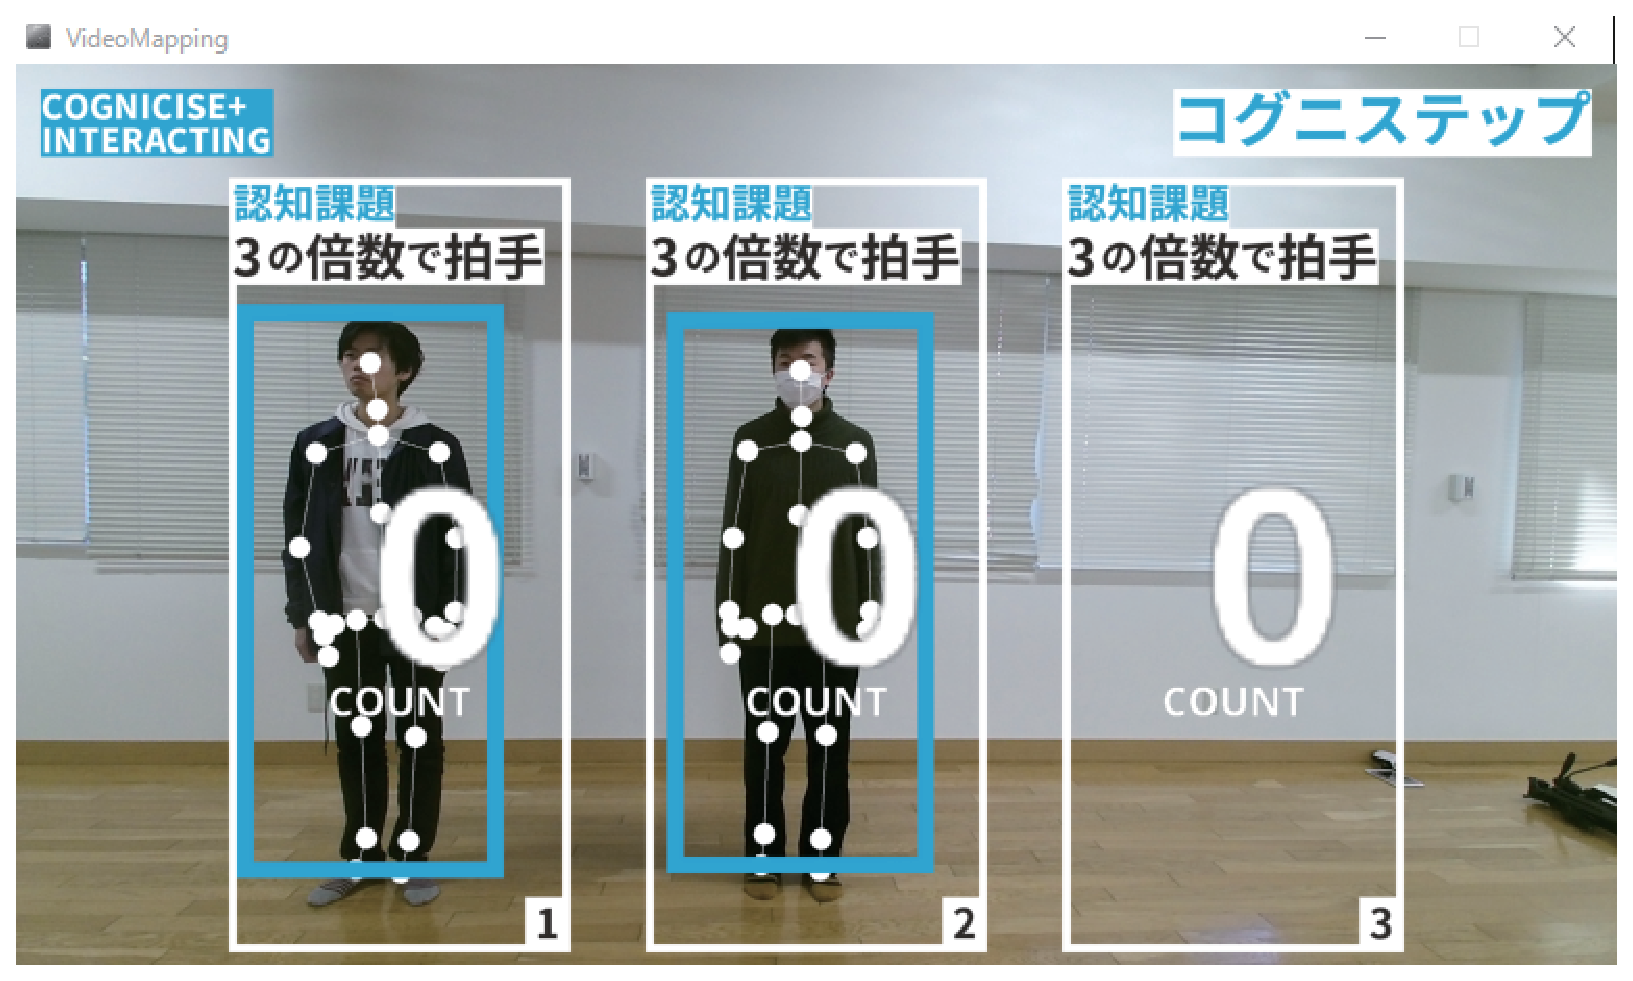
\includegraphics[width=.40\textwidth]{vm_init.eps}
\caption{プロジェクタ投影面(赤枠内が認知課題)}
\label{fig:projection_surface}
\end{center}
\end{figure}

\begin{figure}[tbp]
\begin{center}
\includegraphics[width=.40\textwidth]{db_init.eps}
\caption{PC上のシステムの管理画面(赤枠内で認知課題の変更が可能)}
\label{fig:system_management}
\end{center}
\end{figure}

\begin{figure}[tbp]
\begin{center}
\includegraphics[width=.40\textwidth]{db_user_info.eps}
\caption{PC上のシステムの管理画面(赤枠内が認知課題の正答率)}
\label{fig:check_answer_rate}
\end{center}
\end{figure}


%--------------------------------------------
\section{実験と考察}
提案システムを使用したアンケート評価を行った.評価対象は,参加者のみでコグニステップを実施する実験 (実験1),提案システムを使用してコグニステップを実施する実験 (実験2)の2種類を用意した.60代から70代の高齢者4名に対して5段階の単一回答形式と自由記述式のアンケートを用いた. 

\begin{figure}[b]
\begin{center}
\includegraphics[width=.4\textwidth]{use_system.eps}
\caption{実験の様子}
\label{fig:db_init}
\end{center}
\end{figure}

%--------------------------------------------
\section{まとめ}


%--------------------------------------------

\begin{thebibliography}{9}

\bibitem{コグニサイズとは}
国立長寿医療研究センター: ``コグニサイズとは?'', \url{http://www.ncgg.go.jp/cgss/department/cre/cognicise.html}

% \bibitem{認知症予防へ向けた運動コグニサイズ}
% 国立長寿医療研究センター: ``認知症予防へ向けた運動コグニサイズ'', \url{http://www.ncgg.go.jp/cgss/department/cre/documents/cogni.pdf}

% \bibitem{認知症予防マニュアル}
% 国立長寿医療研究センター: ``認知症予防マニュアル'', pp. 6--8 (2011)

\bibitem{運動教室の効果}
滝本幸治, 宮本謙三, 竹林秀晃, 井上佳和, 宅間豊, 古谷信之, 宮本祥子, 岡部孝生: ``地域に根ざした高齢者運動教室の効果検証'', 理学療法学, Vol. 24, No. 2, pp. 281--285 (2009)

\bibitem{認知課題ゲーム}
北越大輔: ``ヒューマン・ロボット・インタラクションを用いた対戦型ゲームによる介護予防システム'', 科学研究費助成事業 研究成果報告書 (2014)

\end{thebibliography}
\end{document}

%%% Local Variables: 
%%% mode: japanese-latex
%%% TeX-master: t
%%% End: 
